\documentclass{standalone}
\usepackage{tikz}
\usepackage{amsmath}
\usepackage{graphicx}
\usetikzlibrary{positioning, shapes.geometric, shapes.multipart, arrows.meta, calc, fit}

% Global layout controls
\def\mainNodeSep{0.95cm}
\def\rowGap{0.42cm}
\def\colGap{0.9cm}
\def\legendOffsetX{1.2cm}
\def\legendPanelW{14.8cm}
\def\legendPanelH{10.2cm}
\def\legendPadX{0.6cm}
\def\legendTopInset{1.6cm}
\def\legendBottomInset{1.0cm}
\def\curveRound{5pt}

\newcommand{\MMMLSharedStyles}{
  \tikzset{
    basebox/.style={
      rectangle,
      rounded corners=2.5pt,
      draw=black!70,
      minimum height=0.95cm,
      minimum width=2.1cm,
      align=center
    },
    dense/.style={basebox, fill=orange!25,  minimum height=1.0cm, minimum width=1.2cm, text width=1.9cm},
    process/.style={dense},
    process2/.style={basebox, fill=orange!15, minimum height=0.8cm, text width=3.9cm},
    silu/.style={
      circle, draw=black!70, fill=white, minimum size=1.0cm,
      path picture={
        \draw[-, line width=0.9pt] (path picture bounding box.center) circle (0.28cm);
        \begin{scope}
          \clip (path picture bounding box.center) circle (0.28cm);
          \draw[-, domain=-2:2,smooth,variable=\x,line width=0.7pt]
            plot ({0.11*\x},{0.11*(\x/(1+exp(-\x)))});
        \end{scope}
      }
    },
    plusop/.style={
      circle, draw=black!70, fill=white, minimum size=1cm,
      path picture={
        \draw[-, line width=0.9pt]
          (path picture bounding box.west) -- (path picture bounding box.east);
        \draw[-, line width=0.9pt]
          (path picture bounding box.south) -- (path picture bounding box.north);
      }
    },
    basis/.style={basebox, fill=cyan!25, minimum height=1.0cm, minimum width=3.2cm},
    message/.style={basebox, fill=green!30, minimum height=1.2cm, minimum width=4.2cm},
    tensor/.style={basebox, fill=red!25, minimum height=1.2cm, minimum width=2.2cm},
    extra/.style={basebox, fill=gray!25, minimum height=1.2cm, minimum width=2.2cm},
    embedding/.style={basebox, fill=blue!25, minimum height=1.2cm, minimum width=4.2cm},
    output/.style={basebox, fill=yellow!25, minimum height=0.95cm, minimum width=0.8cm, align=center, font=\sffamily\Large},
    legendbox/.style={rectangle, draw=black!60, rounded corners=1.5pt, minimum width=0.8cm, minimum height=0.55cm},
    legendtext/.style={anchor=west, font=\sffamily\Large, align=left, text width=12.8cm}
  }
}


\begin{document}
\resizebox{\textwidth}{!}{%
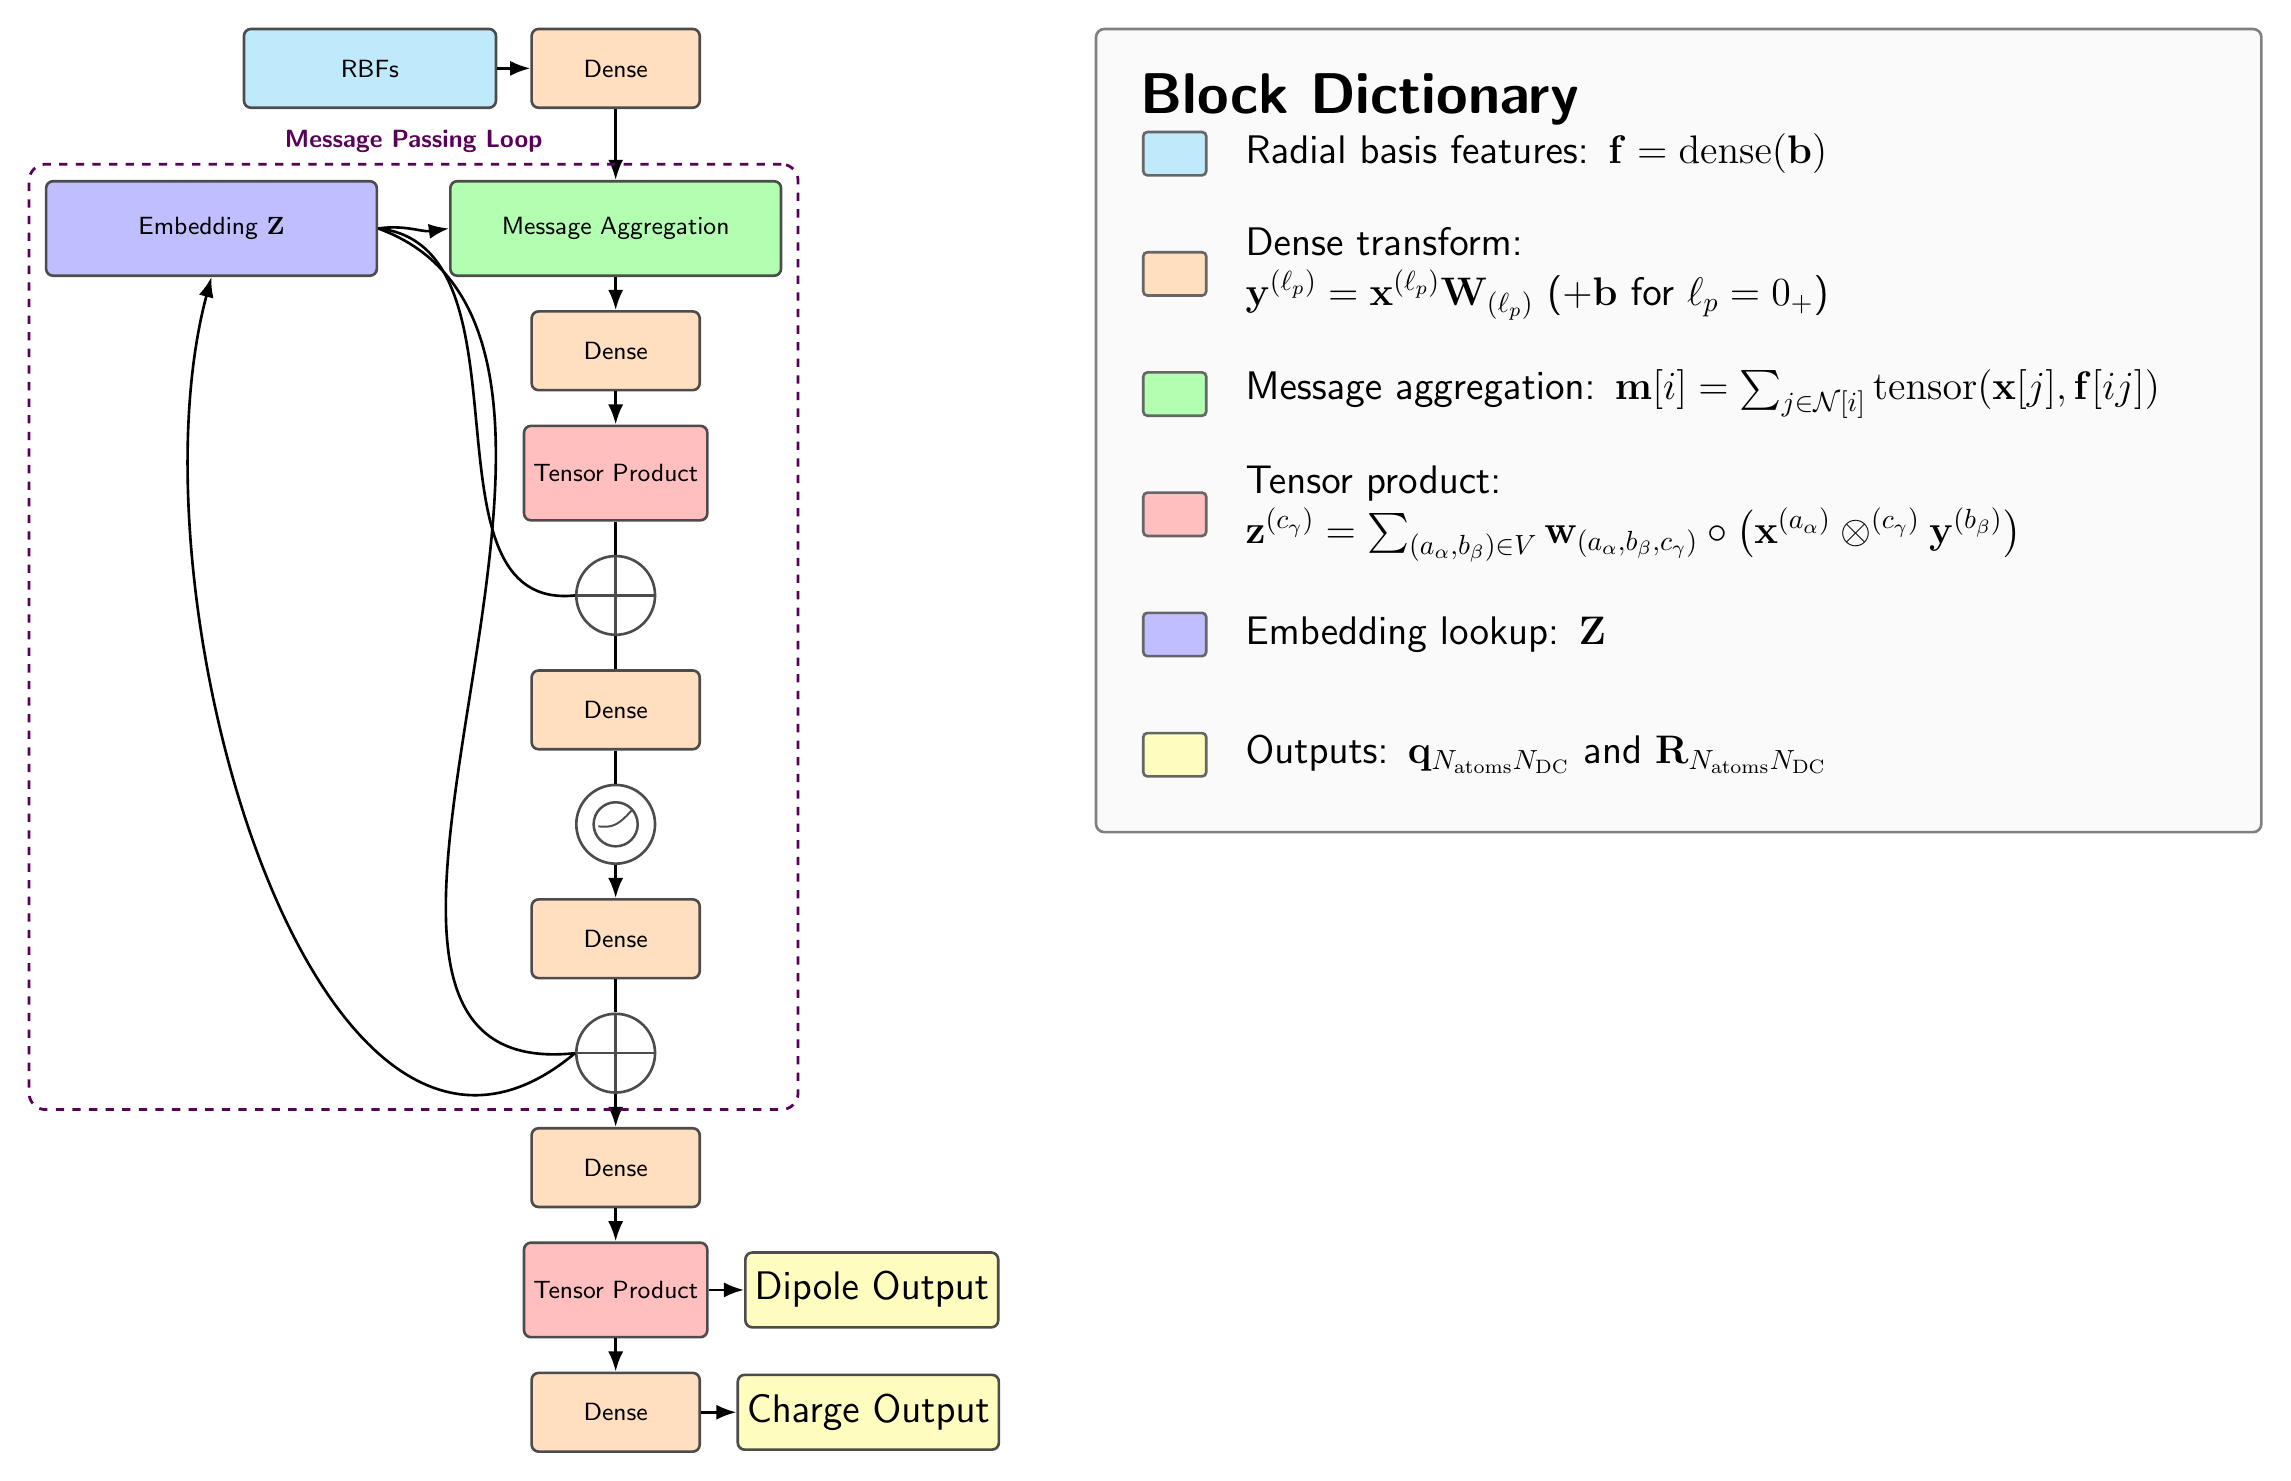
\begin{tikzpicture}[
  auto,
  node distance=\mainNodeSep and \mainNodeSep,
  line width=0.95pt,
  >=Latex,
  ->,
  font=\sffamily\small
]

    \MMMLSharedStyles

    \node[dense] (basis)
    {Dense};
    
    %\node[message, below=0.5cm of basis] (message1)
    %{$\mathbf{f} = \mathrm{dense}(\mathbf{b})$};

    
    \node[message, below=\colGap of basis] (message2)
    {Message Aggregation};
    
    \node[embedding, left=\colGap of message2] (embedding)
    {Embedding $\mathbf{Z}$};
    

    \node[dense, below=\rowGap of message2] (dense)
    {Dense};

    \node[basis, above=\rowGap of embedding, left=\rowGap of basis] (rbf)
    {RBFs};

    \draw[->] (rbf) -- (basis);

    \draw[->] (basis) -- (message2);
    

    \node[tensor, below=\rowGap of dense] (tensor1)
    {Tensor Product};
    

    \draw[->] (embedding.east) to[out=8,in=188] (message2.west);
    \draw[->] (message2) -- (dense);
    \draw[->] (dense) -- (tensor1);

    \node[plusop, below=\rowGap of tensor1] (po1) {};

    \draw[-] (tensor1) -- (po1);
    \draw[-] (embedding.east) to[out=-6,in=186] (po1.west);

    \node[dense, below=\rowGap of po1] (dense2) 
    {Dense};


    \draw[-] (po1) -- (dense2);

    \node[silu, below=\rowGap of dense2] (silu1) {};
    
    \draw[-] (dense2) -- (silu1);

    \node[dense, below=\rowGap of silu1] (dense3) 
    {Dense};


    \draw[->] (silu1) -- (dense3) {};

    \node[plusop, below=\rowGap of dense3] (po2) {};

    \draw[-] (dense3) -- (po2) {};
    \draw[-] (embedding.east) to[out=-20,in=186] (po2.west) {};
    \draw[->] (po2.west) to[out=220,in=-105] (embedding.south) {};

    \node[dense, below=\rowGap of po2] (dense4) 
    {Dense};
    
    \draw[->] (po2) -- (dense4) {};
    

    \node[tensor, below=\rowGap of dense4] (tensor2)
    {Tensor Product};

    \draw[->] (dense4) -- (tensor2) {};

    
    \node[dense, below=\rowGap of tensor2] (dense6) 
    {Dense};
 
    \draw[->] (tensor2) -- (dense6);

    \node[output, right=0.45cm of dense6] (mono)
    {Charge Output};

    \node[output, right=0.45cm of tensor2] (dipo)
    {Dipole Output};

    \draw[->] (tensor2) -- (dipo);
    \draw[->] (dense6) -- (mono);

    % Message passing loop highlight
    \node[draw=violet!70!black, rounded corners=6pt, dashed, line width=1.0pt, inner sep=0.2cm,
      fit=(embedding) (message2) (tensor1) (po1) (dense2) (silu1) (dense3) (po2)] (mploop) {};
    \node[anchor=south, font=\sffamily\small\bfseries, text=violet!70!black] at (mploop.north) {Message Passing Loop};

    % Color dictionary / legend
    \path (current bounding box.north east) coordinate (figNE);
    \node[draw=black!50, rounded corners=3pt, fill=black!2, minimum width=\legendPanelW, minimum height=\legendPanelH, anchor=north west]
      (legendpanel) at ($(figNE)+(\legendOffsetX,0)$) {};
    \coordinate (legStart) at ($(legendpanel.north west)+(\legendPadX,-\legendTopInset)$);
    \coordinate (legEnd) at ($(legendpanel.south west)+(\legendPadX,\legendBottomInset)$);
    \coordinate (leg2) at ($(legStart)!0.2!(legEnd)$);
    \coordinate (leg3) at ($(legStart)!0.4!(legEnd)$);
    \coordinate (leg4) at ($(legStart)!0.6!(legEnd)$);
    \coordinate (leg5) at ($(legStart)!0.8!(legEnd)$);
    \node[anchor=north west, font=\sffamily\bfseries\huge] (legendtitle) at ($(legendpanel.north west)+(0.45,-0.45)$) {Block Dictionary};
    \node[legendbox, fill=cyan!25, anchor=west] (lg1) at (legStart) {};
    \node[legendtext, right=0.35cm of lg1.east, anchor=west] {Radial basis features: $\mathbf{f}=\mathrm{dense}(\mathbf{b})$};
    \node[legendbox, fill=orange!25, anchor=west] (lg2) at (leg2) {};
    \node[legendtext, right=0.35cm of lg2.east, anchor=west] {Dense transform:\\$\mathbf{y}^{(\ell_p)}=\mathbf{x}^{(\ell_p)}\mathbf{W}_{(\ell_p)}$ (+$\mathbf{b}$ for $\ell_p=0_+$)};
    \node[legendbox, fill=green!30, anchor=west] (lg3) at (leg3) {};
    \node[legendtext, right=0.35cm of lg3.east, anchor=west] {Message aggregation: $\mathbf{m}[i]=\sum_{j\in\mathcal{N}[i]}\mathrm{tensor}(\mathbf{x}[j],\mathbf{f}[ij])$};
    \node[legendbox, fill=red!25, anchor=west] (lg4) at (leg4) {};
    \node[legendtext, right=0.35cm of lg4.east, anchor=west] {Tensor product:\\$\mathbf{z}^{(c_\gamma)}=\sum_{(a_\alpha,b_\beta)\in V}\mathbf{w}_{(a_\alpha,b_\beta,c_\gamma)}\circ\left(\mathbf{x}^{(a_\alpha)}\otimes^{(c_\gamma)}\mathbf{y}^{(b_\beta)}\right)$};
    \node[legendbox, fill=blue!25, anchor=west] (lg5) at (leg5) {};
    \node[legendtext, right=0.35cm of lg5.east, anchor=west] {Embedding lookup: $\mathbf{Z}$};
    \node[legendbox, fill=yellow!25, anchor=west] (lg6) at (legEnd) {};
    \node[legendtext, right=0.35cm of lg6.east, anchor=west] {Outputs: $\mathbf{q}_{N_{\mathrm{atoms}}N_{\mathrm{DC}}}$ and $\mathbf{R}_{N_{\mathrm{atoms}}N_{\mathrm{DC}}}$};
    %
    %% Nodes inside the process block
    %\node[circleop, below left=0.5cm and 0.5cm of message.north] (circ1) {};
    %\node[circleop, below right=1cm and 0.5cm of circ1] (circ2) {};
    %\node[block, right=1.2cm of circ1] (linear) {Linear};
    %
    %% External Inputs
    %\node[above left=1.2cm and 1cm of circ1] (rji) {$R(r_{ji})$};
    %\node[above right=1.2cm and 0.5cm of linear] (hi) {$h_i^{(t)}$};
    %\node[left=2.5cm of circ2] (ylm) {$Y^l_m(\hat{r}_{ji})$};
    %\node[left=1.0cm of circ1] (negzi) {$-z_i$};
    %\node[right=1.0cm of hi] (xi) {$x_i$};
    %\node[below=1.0cm of circ2] (mji) {$m_{ji}^{(t)}$};

    %% Connections
    %\draw[->] (rji) -- (circ1);
    %\draw[->] (hi) -- (linear);
    %\draw[->] (linear.west) -- ++(-0.5,0) |- (circ2);
    %\draw[->] (circ1) -- ++(0.5,0) |- (circ2);
    %\draw[->] (circ2) -- (mji);
    %\draw[->] (ylm) -- (circ2);
    %\draw[->] (negzi) -- (circ1);
    %\draw[->] (xi) |- (linear.east);

    %% Main interaction block
    %\node[interaction, below=3.5cm of message] (interaction) {};
    %\node[above=0.3cm of interaction.north] {};

    %% Sub-blocks inside interaction
    %\node[message, above=0.3cm of interaction.south] (message) {Message};
    %\node[update, below=0.3cm of interaction.north] (update) {Update};

    %% External Inputs and Outputs
    %\node[left=1cm of message.west] (rji) {$R(r_{ji})$};
    %\node[left=1cm of update.west] (ylm) {$Y^l_m(\hat{r}_{ji})$};
    %\node[above=0.3cm of interaction.north] (hti) {$h_i^{(t)}$};
    %\node[right=1.5cm of interaction.east] (zi) {$z_i$};
    %\node[right=1cm of update.east] (mji) {$m_{ji}^{(t)}$};
    %\node[below=0.5cm of update.south] (hti1) {$h_i^{(t+1)}$};

    % Connections
    %\draw[->] (rji) -- (message.west);
    %\draw[->] (ylm) -- (message.west);
    %\draw[->] (message.east) -- ++(0.5,0) |- (update.east);
    %\draw[->] (message.east) -- (mji);
    %\draw[->] (hti) -- (interaction.north);
    %\draw[->] (update.west) -- ++(-0.5,0) |- (hti1);
    %\draw[->] (zi) -- ++(-0.5,0) |- (interaction.east);
    %\draw[->] (zi) -- ++(-0.5,0) |- (update.east);
    %\draw[->] (interaction.east) -- (zi);
    
\end{tikzpicture}%
}


% \begin{split}\mathbf{y}^{(\ell_p)} = \begin{cases}
% \mathbf{x}^{(\ell_p)}\mathbf{W}_{(\ell_p)} + \mathbf{b} & \ell_p = 0_+ \\
% \mathbf{x}^{(\ell_p)}\mathbf{W}_{(\ell_p)} & \ell_p \neq 0_+
% \end{cases}\end{split}

\end{document}


